\documentclass{article}

% content/resources/templates/preamble.tex
\usepackage[margin=0.6in]{geometry}
\author{Milav Dabgar}
\usepackage{amsmath,amssymb,amsthm}
\usepackage{booktabs}
\usepackage{multirow}
\usepackage{xcolor}
\usepackage{tcolorbox}
\tcbuselibrary{breakable,skins}
\usepackage[colorlinks=true,linkcolor=blue]{hyperref}
\usepackage{titlesec}
\usepackage{enumitem}
\usepackage{tikz}
\usepackage{pgfplots}
\usepackage{circuitikz}
\usepackage[version=4]{mhchem}
\usepackage{longtable}
\usepackage{array}
\usepackage{float}
\usepackage{caption}
\usepackage{listings}

\lstset{
  basicstyle=\small\ttfamily,
  breaklines=true,
  breakatwhitespace=false,
  postbreak=\mbox{\textcolor{red}{$\hookrightarrow$}\space},
  float=false,
  numbers=left,
  numberstyle=\tiny\color{gray},
  numbersep=10pt,
  xleftmargin=2em,
  keywordstyle=\color{blue},
  commentstyle=\color{green!60!black},
  stringstyle=\color{purple},
  backgroundcolor=\color{gray!5},
  showstringspaces=false,
  tabsize=2,
  captionpos=b,
  keepspaces=true,
  columns=flexible
}

\pgfplotsset{compat=1.18}
\usetikzlibrary{shapes,arrows,positioning,calc,patterns,decorations.pathmorphing,decorations.markings,arrows.meta}

% Color scheme
\definecolor{headcolor}{RGB}{0,102,204}
\definecolor{keycolor}{RGB}{220,20,60}
\definecolor{solutioncolor}{RGB}{34,139,34}
\definecolor{mnemoniccolor}{RGB}{148,0,211}
\definecolor{codecolor}{RGB}{0,0,100}

% Spacing
\setlength{\parskip}{3pt}
\setlist[itemize]{nosep}
\setlist[enumerate]{nosep}

% Title formatting
\titleformat{\section}{\Large\bfseries\color{headcolor}}{\thesection}{1em}{}
\titleformat{\subsection}{\large\bfseries\color{headcolor}}{\thesubsection}{1em}{}

% Pandoc tightlist compatibility
\providecommand{\tightlist}{%
  \setlength{\itemsep}{0pt}\setlength{\parskip}{0pt}}

% Pandoc longtable compatibility
\newcounter{none}
\def\thenone{}


% content/resources/templates/english-boxes.tex

% Custom environments
\newtcolorbox{solutionbox}{
 breakable,
 enhanced,
 colback=solutioncolor!5!white,
 colframe=solutioncolor!75!black,
 fonttitle=\bfseries,
 title=Solution
}

\newtcolorbox{solutionboxnobreak}{
 colback=solutioncolor!5!white,
 colframe=solutioncolor!75!black,
 fonttitle=\bfseries,
 title=Solution
}

\newtcolorbox{keyformula}{
 breakable,
 enhanced,
 colback=keycolor!5!white,
 colframe=keycolor!75!black,
 fonttitle=\bfseries,
 title=Key Formula
}

\newtcolorbox{mnemonicboxenv}{
 breakable,
 enhanced,
 colback=mnemoniccolor!5!white,
 colframe=mnemoniccolor!75!black,
 fonttitle=\bfseries,
 title=Mnemonic
}

\newcommand{\mnemonicbox}[1]{%
  \begin{mnemonicboxenv}
    #1
  \end{mnemonicboxenv}
}


% Custom commands for GTU solutions
% This file defines semantic commands for consistent formatting

% Question command with automatic formatting
\newcommand{\question}[2]{%
  \section*{Question #1}%
  \textbf{#2}%
}

% OR question variant
\newcommand{\questionor}[2]{%
  \section*{Question #1 OR}%
  \textbf{#2}%
}

% Proper table environment with caption
\newenvironment{answertable}[1]{%
  \begin{table}[htbp]
  \centering
  \caption{#1}
}{%
  \end{table}
}

% Proper figure environment for diagrams
\newenvironment{answerdiagram}[1]{%
  \begin{figure}[htbp]
  \centering
  \caption{#1}
}{%
  \end{figure}
}

% Semantic markup for key terms
\newcommand{\keyword}[1]{\textbf{#1}}
\newcommand{\code}[1]{\texttt{#1}}
\newcommand{\classname}[1]{\texttt{#1}}
\newcommand{\methodname}[1]{\texttt{#1}}

% Proper quotation marks
\newcommand{\mnemonic}[1]{``#1''}


\title{Principles of Electronic Communication (4331104) - Summer 2023 Solution}
\date{July 25, 2023}

\begin{document}
\maketitle

\questionmarks{1}{a}{3}
\textbf{Draw \& explain block diagram of Communication system.}

\begin{solutionbox}
\textbf{Block Diagram of Communication System:}

\begin{center}
\begin{tikzpicture}[auto, node distance=2cm, >=latex]
    \node [gtu block] (source) {Input Source};
    \node [gtu block, right of=source, node distance=3cm] (tx) {Transmitter};
    \node [gtu block, right of=tx, node distance=3cm] (channel) {Channel};
    \node [gtu block, right of=channel, node distance=3cm] (rx) {Receiver};
    \node [gtu block, right of=rx, node distance=3cm] (dest) {Output};
    \node [gtu block, below of=channel, node distance=2cm] (noise) {Noise Source};

    \draw [gtu arrow] (source) -- (tx);
    \draw [gtu arrow] (tx) -- (channel);
    \draw [gtu arrow] (channel) -- (rx);
    \draw [gtu arrow] (rx) -- (dest);
    \draw [gtu arrow] (noise) -- (channel);
\end{tikzpicture}
\captionof{figure}{Block Diagram of Communication System}
\end{center}

\begin{itemize}
    \item \textbf{Input}: Message signal originating from source (e.g., voice, picture, data).
    \item \textbf{Transmitter}: Converts message to suitable form for transmission (modulation, amplification).
    \item \textbf{Channel}: Medium through which signal travels (e.g., wire, fiber, free space).
    \item \textbf{Receiver}: Extracts original message from received signal (demodulation, amplification).
    \item \textbf{Output}: Delivered message to destination.
    \item \textbf{Noise Source}: Unwanted signals that interfere with communication, adding distortion.
\end{itemize}
\end{solutionbox}

\begin{mnemonicbox}
\mnemonic{I Transmit Clearly Receiving Original Messages}
\end{mnemonicbox}

\questionmarks{1}{b}{4}
\textbf{Explain need of modulation. State advantages of modulation.}

\begin{solutionbox}
\textbf{Need for Modulation:}

\begin{center}
\begin{tikzpicture}[node distance=2cm]
    \node (center) [gtu block] {Modulation};
    \node (ant) [gtu state, above of=center] {Practical Antenna Size};
    \node (mux) [gtu state, right of=center, xshift=2cm] {Multiplexing};
    \node (noise) [gtu state, below of=center] {Noise Reduction};
    \node (range) [gtu state, left of=center, xshift=-2cm] {Transmission Range};

    \draw [gtu arrow] (ant) -- (center);
    \draw [gtu arrow] (mux) -- (center);
    \draw [gtu arrow] (noise) -- (center);
    \draw [gtu arrow] (range) -- (center);
\end{tikzpicture}
\end{center}

\textbf{Advantages of Modulation:}

\begin{enumerate}
    \item \textbf{Reduced antenna size}: 
    \begin{itemize}
        \item Antenna height $h = \lambda/4 = c/4f$.
        \item For audio frequencies (low $f$), $h$ is impractically large (km).
        \item Modulation shifts signal to high $f$, reducing required antenna size to meters.
    \end{itemize}
    \item \textbf{Multiplexing possible}: 
    \begin{itemize}
        \item Multiple signals can be transmitted simultaneously through the same channel by assigning different carrier frequencies.
    \end{itemize}
    \item \textbf{Increased range}: 
    \begin{itemize}
        \item Low frequency baseband signals suffer high attenuation.
        \item Modulated high frequency signals travel farther with less attenuation.
    \end{itemize}
    \item \textbf{Noise reduction}: 
    \begin{itemize}
        \item Modulation techniques (like FM, PCM) offer better immunity to noise compared to baseband transmission, improving SNR.
    \end{itemize}
\end{enumerate}
\end{solutionbox}

\begin{mnemonicbox}
\mnemonic{Antennas Need Modulation For Reaching Anywhere with Noise Immunity}
\end{mnemonicbox}

\questionmarks{1}{c}{7}
\textbf{Define modulation. Explain Amplitude modulation with waveform and derive voltage equation for modulated signal.}

\begin{solutionbox}
\textbf{Modulation}: The process of varying a fundamental parameter (amplitude, frequency, or phase) of a high-frequency carrier signal proportionally to the instantaneous value of the low-frequency message signal.

\textbf{Amplitude Modulation Waveform:}

\begin{center}
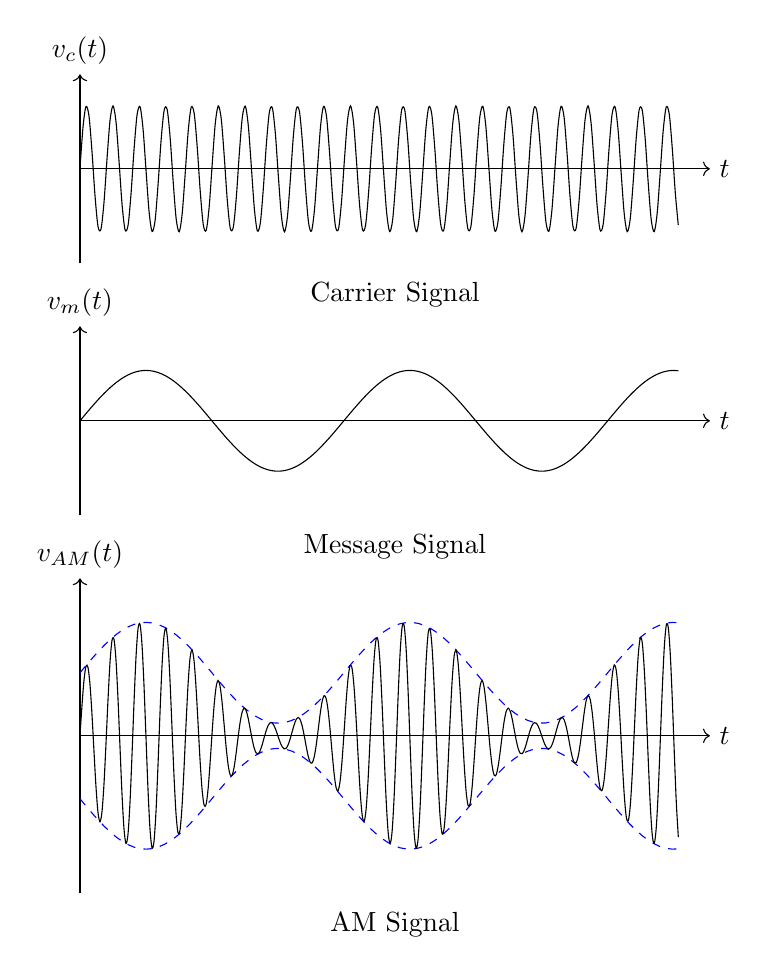
\begin{tikzpicture}[scale=0.8]
    % Carrier
    \begin{scope}[yshift=4cm]
        \draw[->] (0,0) -- (10,0) node[right] {$t$};
        \draw[->] (0,-1.5) -- (0,1.5) node[above] {$v_c(t)$};
        \draw[domain=0:9.5, samples=200, smooth] plot (\x, {1*sin(15*\x r)});
        \node at (5,-2) {Carrier Signal};
    \end{scope}

    % Message
    \begin{scope}[yshift=0cm]
        \draw[->] (0,0) -- (10,0) node[right] {$t$};
        \draw[->] (0,-1.5) -- (0,1.5) node[above] {$v_m(t)$};
        \draw[domain=0:9.5, samples=100, smooth] plot (\x, {0.8*sin(1.5*\x r)});
        \node at (5,-2) {Message Signal};
    \end{scope}

    % AM Signal
    \begin{scope}[yshift=-5cm]
        \draw[->] (0,0) -- (10,0) node[right] {$t$};
        \draw[->] (0,-2.5) -- (0,2.5) node[above] {$v_{AM}(t)$};
        % Envelope
        \draw[dashed, blue] plot[domain=0:9.5, samples=100] (\x, {1 + 0.8*sin(1.5*\x r)});
        \draw[dashed, blue] plot[domain=0:9.5, samples=100] (\x, {-(1 + 0.8*sin(1.5*\x r))});
        % Signal
        \draw[domain=0:9.5, samples=300, smooth] plot (\x, {(1 + 0.8*sin(1.5*\x r)) * sin(15*\x r)});
        \node at (5,-3) {AM Signal};
    \end{scope}
\end{tikzpicture}
\captionof{figure}{Amplitude Modulation Waveforms}
\end{center}

\textbf{Derivation of AM Voltage Equation:}

\begin{enumerate}
    \item Let the instantaneous value of carrier signal be:
    \[ v_c(t) = V_c \sin(\omega_c t) \]
    
    \item Let the instantaneous value of modulating (message) signal be:
    \[ v_m(t) = V_m \sin(\omega_m t) \]
    
    \item In AM, the amplitude of the carrier $V_c$ is varied in accordance with the message signal $v_m(t)$. The instantaneous amplitude of the modulated wave $A(t)$ becomes:
    \[ A(t) = V_c + v_m(t) = V_c + V_m \sin(\omega_m t) \]
    \[ A(t) = V_c [1 + \frac{V_m}{V_c} \sin(\omega_m t)] \]
    
    \item Define \textbf{Modulation Index} ($\mu$):
    \[ \mu = \frac{V_m}{V_c} \]
    So, $A(t) = V_c [1 + \mu \sin(\omega_m t)]$
    
    \item The instantaneous value of the AM wave $v_{AM}(t)$ is given by:
    \[ v_{AM}(t) = A(t) \sin(\omega_c t) \]
    
    \item Substituting $A(t)$:
    \[ v_{AM}(t) = V_c [1 + \mu \sin(\omega_m t)] \sin(\omega_c t) \]
    This is the standard equation for an AM signal.
\end{enumerate}
\end{solutionbox}

\begin{mnemonicbox}
\mnemonic{Amplitude Modulation Makes Carrier Value Change}
\end{mnemonicbox}

\questionmarks{1}{c}{7}
\textbf{OR: Define noise. Give classification of noise and explain cause of any three internal noise.}

\begin{solutionbox}
\textbf{Noise}: Unwanted electrical signals that interfere with the transmission and processing of desired communication signals, causing distortion, errors, or loss of information.

\textbf{Classification of Noise:}

\begin{center}
\begin{tabulary}{\linewidth}{|L|L|}
\hline
\textbf{External Noise} & \textbf{Internal Noise} \\ \hline
Atmospheric Noise & Thermal (Johnson) Noise \\ 
Extraterrestrial (Solar/Cosmic) Noise & Shot Noise \\ 
Industrial (Man-made) Noise & Transit-time Noise \\ 
 & Flicker (1/f) Noise \\ 
 & Partition Noise \\ \hline
\end{tabulary}
\captionof{table}{Classification of Noise}
\end{center}

\textbf{Causes of Internal Noise:}

\begin{enumerate}
    \item \textbf{Thermal (Johnson) Noise}:
    \begin{itemize}
        \item \textbf{Cause}: Generated by the random thermal motion of free electrons inside a conductor or resistor.
        \item \textbf{Characteristic}: It is present in all resistive components and is directly proportional to absolute temperature ($T$) and bandwidth ($B$).
        \item Power $P_n = kTB$.
    \end{itemize}
    
    \item \textbf{Shot Noise}:
    \begin{itemize}
        \item \textbf{Cause}: Arises from the discrete nature of charge carriers (electrons/holes). It occurs due to the random fluctuations in the arrival rate of carriers crossing a potential barrier (e.g., in PN junctions, vacuum tubes).
        \item \textbf{Characteristic}: It is present in active devices like diodes and transistors. It is proportional to the DC current flowing through the device.
    \end{itemize}
    
    \item \textbf{Flicker Noise (1/f Noise)}:
    \begin{itemize}
        \item \textbf{Cause}: Caused by variations in carrier density due to surface defects, contamination, and impurities in semiconductor materials.
        \item \textbf{Characteristic}: Its power spectral density is inversely proportional to frequency ($1/f$), making it significant at low frequencies (below a few kHz).
    \end{itemize}
\end{enumerate}
\end{solutionbox}

\begin{mnemonicbox}
\mnemonic{This Shooting Flicker Is Noisy Everywhere}
\end{mnemonicbox}

\questionmarks{2}{a}{3}
\textbf{Define (1) Modulation index for AM (2) Noise Figure (3) Digital Modulation}

\begin{solutionbox}
\begin{enumerate}
    \item \textbf{Modulation Index for AM ($\mu$)}:
    \begin{itemize}
        \item Defined as the ratio of the peak amplitude of the modulating signal ($V_m$) to the peak amplitude of the carrier signal ($V_c$).
        \item Formula: $\mu = \frac{V_m}{V_c}$
        \item Practical range: $0 \le \mu \le 1$ to avoid overmodulation distortion.
    \end{itemize}
    
    \item \textbf{Noise Figure (NF)}:
    \begin{itemize}
        \item A figure of merit that indicates how much noise a device (like an amplifier) adds to a signal.
        \item Defined as the ratio of input Signal-to-Noise Ratio (SNR) to output Signal-to-Noise Ratio.
        \item Formula: $NF = \frac{(SNR)_{input}}{(SNR)_{output}}$
        \item Ideally $NF=1$ (or 0 dB) for a noise-free device. Always $\ge 1$ in practice.
    \end{itemize}
    
    \item \textbf{Digital Modulation}:
    \begin{itemize}
        \item A technique where digital data (binary 0s and 1s) is used to modulate the parameters (amplitude, frequency, or phase) of an analog carrier signal for transmission.
        \item Examples: ASK (Amplitude Shift Keying), FSK (Frequency Shift Keying), PSK (Phase Shift Keying).
    \end{itemize}
\end{enumerate}
\end{solutionbox}

\begin{mnemonicbox}
\mnemonic{Modulation Measures, Noise Numbers, Digital Data}
\end{mnemonicbox}

\questionmarks{2}{b}{4}
\textbf{Derive equation for total power transmitted for amplitude modulated signal considering carrier power and modulation index.}

\begin{solutionbox}
\textbf{Derivation of Total Power in AM:}

\begin{enumerate}
    \item The equation for an AM wave is:
    \[ v_{AM}(t) = V_c \sin(\omega_c t) + \frac{\mu V_c}{2} \cos(\omega_c - \omega_m)t - \frac{\mu V_c}{2} \cos(\omega_c + \omega_m)t \]
    It consists of a Carrier component and two Sideband components (LSB and USB).
    
    \item Power is given by $P = \frac{V_{rms}^2}{R}$. Assuming load resistance $R$:
    
    \item \textbf{Carrier Power ($P_c$)}:
    Peak voltage is $V_c$, so $V_{rms} = \frac{V_c}{\sqrt{2}}$.
    \[ P_c = \frac{(V_c/\sqrt{2})^2}{R} = \frac{V_c^2}{2R} \]
    
    \item \textbf{Sideband Power}:
    Both LSB and USB have peak amplitude $\frac{\mu V_c}{2}$.
    \[ V_{sb\_rms} = \frac{\mu V_c}{2\sqrt{2}} \]
    Power in Upper Sideband ($P_{USB}$) = Power in Lower Sideband ($P_{LSB}$):
    \[ P_{SB} = \frac{(\frac{\mu V_c}{2\sqrt{2}})^2}{R} = \frac{\mu^2 V_c^2}{8R} \]
    
    \item Substituting $P_c = \frac{V_c^2}{2R}$ into sideband power equation:
    \[ P_{SB} = P_c \cdot \frac{\mu^2}{4} \]
    
    \item \textbf{Total Power ($P_T$)}:
    \[ P_T = P_c + P_{USB} + P_{LSB} \]
    \[ P_T = P_c + P_c \frac{\mu^2}{4} + P_c \frac{\mu^2}{4} \]
    \[ P_T = P_c + P_c \frac{\mu^2}{2} \]
    \[ P_T = P_c \left( 1 + \frac{\mu^2}{2} \right) \]
\end{enumerate}
\end{solutionbox}

\begin{mnemonicbox}
\mnemonic{Power Total = Power Carrier (1 + mu^2/2)}
\end{mnemonicbox}

\questionmarks{2}{c}{7}
\textbf{Explain basic principle of double sideband suppressed carrier amplitude modulation. Derive its voltage equation \& draw only balanced modulator circuit using diode.}

\begin{solutionbox}
\textbf{Double Sideband Suppressed Carrier (DSBSC) Principle:}
\begin{itemize}
    \item In standard AM, the carrier consumes about 67\% of total power but carries no information.
    \item DSBSC suppresses the carrier and transmits only the two sidebands (USB and LSB), which contain the actual information.
    \item \textbf{Advantage}: Improves power efficiency and reduces bandwidth usage per watt of information power.
    \item \textbf{Disadvantage}: Requires complex coherent detection at the receiver.
\end{itemize}

\textbf{Voltage Equation Derivation:}
\begin{enumerate}
    \item Consider carrier $c(t) = V_c \sin(\omega_c t)$ and Message $m(t) = V_m \sin(\omega_m t)$.
    \item DSBSC is the product of carrier and message signals:
    \[ v_{DSBSC}(t) = m(t) \cdot c(t) \]
    \[ v_{DSBSC}(t) = [V_m \sin(\omega_m t)] \cdot [V_c \sin(\omega_c t)] \]
    \[ v_{DSBSC}(t) = V_m V_c \sin(\omega_m t) \sin(\omega_c t) \]
    
    \item Using trigonometric identity: $2 \sin A \sin B = \cos(A-B) - \cos(A+B)$:
    \[ v_{DSBSC}(t) = \frac{V_m V_c}{2} [\cos(\omega_c - \omega_m)t - \cos(\omega_c + \omega_m)t] \]
    
    \item This equation shows two components (LSB and USB) and NO carrier component at $\omega_c$.
\end{enumerate}

\textbf{Balanced Modulator Circuit Using Oscillating Diodes:}

\begin{center}
\begin{circuitikz}[scale=0.9]
    % Transformers
    \draw (0,0) node[transformer] (T1) {};
    \draw (6,0) node[transformer] (T2) {};
    
    % Diodes
    \draw (T1.A1) -- (T1.A2) node[midway, left] {Modulating Signal $v_m(t)$};
    \draw (T1.B1) to[D, l=$D_1$] (T2.A1);
    \draw (T1.B2) to[D, l=$D_2$] (T2.A2);
    
    % Carrier Injection (Center Taps)
    \coordinate (CT1) at ($(T1.B1)!0.5!(T1.B2)$);
    \coordinate (CT2) at ($(T2.A1)!0.5!(T2.A2)$);
    
    \draw (CT1) -- ++(0,-1.5) to[sV, l=Carrier $v_c(t)$] ++(3,0) -- (CT2);
    
    % Output
    \draw (T2.B1) -- (T2.B2) node[midway, right] {Output DSBSC};

    % Connections for transformer symbols
\end{circuitikz}
\captionof{figure}{Ring Modulator / Balanced Modulator using Diodes}
\end{center}
\end{solutionbox}

\begin{mnemonicbox}
\mnemonic{Delete Carrier, Save Bandwidth, Combine Signals}
\end{mnemonicbox}

\questionmarks{2}{a}{3}
\textbf{OR: Define only, w.r.t. radio receiver (1) Sensitivity (2) Selectivity (3) fidelity}

\begin{solutionbox}
\begin{enumerate}
    \item \textbf{Sensitivity}:
    \begin{itemize}
        \item The ability of a radio receiver to pick up weak signals and amplify them to a usable level.
        \item Measured in microvolts ($\mu V$). Lower value means better sensitivity (e.g., a 1 $\mu V$ receiver is more sensitive than a 10 $\mu V$ one).
    \end{itemize}
    
    \item \textbf{Selectivity}:
    \begin{itemize}
        \item The ability of a receiver to select the desired frequency signal while rejecting all other adjacent unwanted signals.
        \item Determined by the quality factor ($Q$) and bandwidth of the tuned circuits. A narrow bandwidth implies high selectivity.
    \end{itemize}
    
    \item \textbf{Fidelity}:
    \begin{itemize}
        \item The ability of a receiver to reproduce all the frequency components of the original message signal in the output without distortion.
        \item High fidelity (Hi-Fi) implies accurate reproduction of the full audio range.
    \end{itemize}
\end{enumerate}
\end{solutionbox}

\begin{mnemonicbox}
\mnemonic{Sensitive Selection Faithfully}
\end{mnemonicbox}

\questionmarks{2}{b}{4}
\textbf{OR: An AM signal has carrier power of 1 KW with 200 watt in each sideband. Find out modulation index.}

\begin{solutionbox}
\textbf{Given:}
\begin{itemize}
    \item Carrier Power ($P_c$) = 1 KW = 1000 W
    \item Power in each sideband ($P_{SB}$) = 200 W (This usually means power in \textit{one} sideband)
\end{itemize}

\textbf{To Find:}
\begin{itemize}
    \item Modulation Index ($\mu$)
\end{itemize}

\textbf{Solution:}
\begin{enumerate}
    \item Total Sideband Power ($P_{TSB}$) is the sum of power in both USB and LSB.
    \[ P_{TSB} = P_{USB} + P_{LSB} = 2 \times P_{SB} \]
    \[ P_{TSB} = 2 \times 200 = 400 \text{ W} \]
    
    \item Formula relating sideband power to carrier power:
    \[ P_{TSB} = P_c \cdot \frac{\mu^2}{2} \]
    Alternatively, using single sideband formula: $P_{SB} = P_c \cdot \frac{\mu^2}{4}$.
    
    \item Substitute values:
    \[ 400 = 1000 \cdot \frac{\mu^2}{2} \]
    
    \item Solve for $\mu^2$:
    \[ \frac{\mu^2}{2} = \frac{400}{1000} = 0.4 \]
    \[ \mu^2 = 0.4 \times 2 = 0.8 \]
    
    \item Solve for $\mu$:
    \[ \mu = \sqrt{0.8} \approx 0.8944 \]
\end{enumerate}

\textbf{Answer:} The modulation index is approximately \textbf{0.89} or \textbf{89.4\%}.
\end{solutionbox}

\questionmarks{2}{c}{7}
\textbf{OR: Compare Amplitude modulation with Frequency Modulation considering minimum seven parameters/aspect.}

\begin{solutionbox}
\begin{center}
\begin{tabulary}{\linewidth}{|L|L|L|}
\hline
\textbf{Parameter} & \textbf{Amplitude Modulation (AM)} & \textbf{Frequency Modulation (FM)} \\ \hline
1. Definition & Amplitude of carrier varies with message amplitude. & Frequency of carrier varies with message amplitude. \\ \hline
2. Modulation Index & $\mu = V_m/V_c$ (Range 0 to 1). & $\beta = \Delta f / f_m$ (Usually $>1$). \\ \hline
3. Bandwidth & Low: $BW = 2f_m$. & High: $BW = 2(f_m + \Delta f)$ (Carson's Rule). \\ \hline
4. Noise Immunity & Poor. Noise affects amplitude directly. & Excellent. Amplitude variations are clipped; frequency carries info. \\ \hline
5. Power Efficiency & Poor. Carrier takes up to 67\% power. & Good. Power is constant and efficient. \\ \hline
6. Complexity & Simple transmitters and receivers. & Complex transmitters and receivers (uses PLL, discriminators). \\ \hline
7. Fidelity (Quality) & Moderate capability. & High fidelity (Hi-Fi), better sound quality. \\ \hline
8. Application & LW/MW/SW Broadcasting, Video transmission. & FM Radio Broadcasting, TV Audio, Satellite. \\ \hline
\end{tabulary}
\captionof{table}{Comparison of AM and FM}
\end{center}
\end{solutionbox}

\questionmarks{3}{a}{3}
\textbf{Draw and label sine wave of 1 KHZ in time domain and frequency domain. State advantage of frequency domain analysis of signal.}

\begin{solutionbox}
\textbf{Time Domain Representation (1 kHz):}
\begin{center}
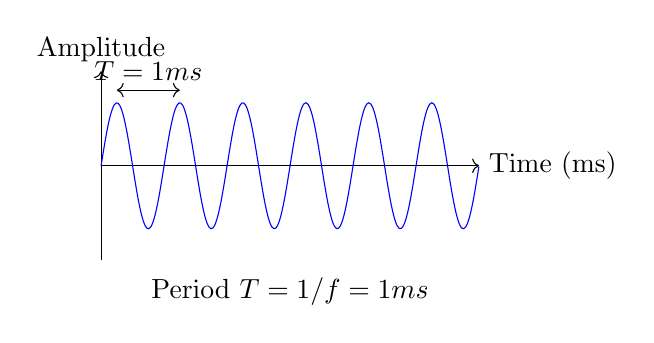
\begin{tikzpicture}[scale=0.8]
    \draw[->] (0,0) -- (6,0) node[right] {Time (ms)};
    \draw[->] (0,-1.5) -- (0,1.5) node[above] {Amplitude};
    \draw[domain=0:6, samples=200, smooth, blue] plot (\x, {sin(360*\x)}); % f=1 means period=1 unit
    \node at (3,-2) {Period $T = 1/f = 1ms$};
    % Mark period
    \draw[<->] (0.25, 1.2) -- (1.25, 1.2) node[midway, above] {$T=1ms$};
\end{tikzpicture}
\end{center}

\textbf{Frequency Domain Representation:}
\begin{center}
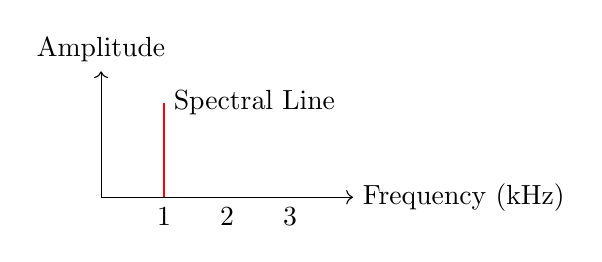
\begin{tikzpicture}[scale=0.8]
    \draw[->] (0,0) -- (4,0) node[right] {Frequency (kHz)};
    \draw[->] (0,0) -- (0,2) node[above] {Amplitude};
    \draw[thick, red] (1,0) -- (1,1.5); % 1 kHz spike
    \node at (1,-0.3) {1};
    \node at (2,-0.3) {2};
    \node at (3,-0.3) {3};
    \node[right] at (1,1.5) {Spectral Line};
\end{tikzpicture}
\end{center}

\textbf{Advantages of Frequency Domain Analysis:}
\begin{itemize}
    \item \textbf{Signal decomposition}: Easily identifies individual frequency components and bandwidth usage.
    \item \textbf{Filter design}: Essential for designing filters (Low Pass, High Pass) as response is defined in frequency.
    \item \textbf{Bandwidth efficiency}: Helps in understanding spectrum occupancy and maximizing channel usage.
\end{itemize}
\end{solutionbox}

\questionmarks{3}{b}{4}
\textbf{State following frequency (1) IF frequency for AM radio (2) IF frequency for FM radio (3) Frequency Band used in FM radio (4) Frequency Band of Human speech.}

\begin{solutionbox}
\begin{center}
\begin{tabulary}{\linewidth}{|L|L|}
\hline
\textbf{Parameter} & \textbf{Standard Frequency Value} \\ \hline
1. IF frequency for AM radio & 455 kHz \\ \hline
2. IF frequency for FM radio & 10.7 MHz \\ \hline
3. Frequency Band used in FM broadcasting & 88 MHz to 108 MHz \\ \hline
4. Frequency Band of Human speech (Voice) & 300 Hz to 3.4 kHz (Telephone standard) \\ \hline
\end{tabulary}
\captionof{table}{Standard Frequencies in Communication}
\end{center}
\end{solutionbox}

\questionmarks{3}{c}{7}
\textbf{Explain Single side band (SSB) modulation with waveform and its advantages. Show how SSB transmission required only 1/6th of power with respect to double sideband full carrier amplitude modulation.}

\begin{solutionbox}
\textbf{Single Sideband (SSB) Modulation:}
\begin{itemize}
    \item SSB is a form of amplitude modulation where the carrier and one of the sidebands are suppressed.
    \item Only \textbf{one sideband} (either Upper Sideband - USB or Lower Sideband - LSB) is transmitted.
    \item This saves bandwidth and power without losing any information.
\end{itemize}

\textbf{SSB Spectrum Waveform:}
\begin{center}
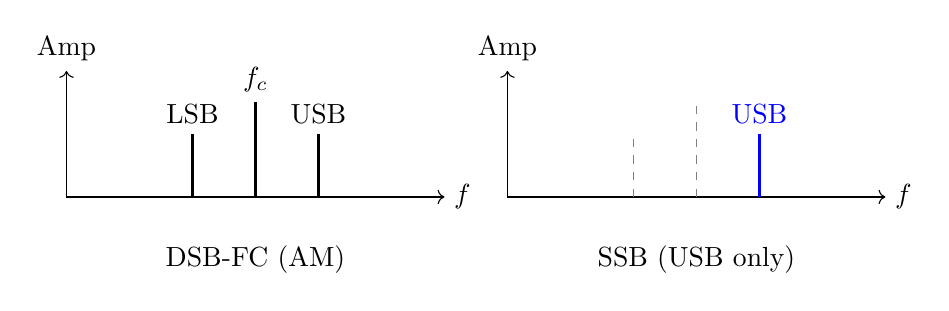
\begin{tikzpicture}[scale=0.8]
    % DSB-FC
    \begin{scope}
        \draw[->] (0,0) -- (6,0) node[right] {$f$};
        \draw[->] (0,0) -- (0,2) node[above] {Amp};
        \draw[thick] (3,0) -- (3,1.5) node[above] {$f_c$}; % Carrier
        \draw[thick] (2,0) -- (2,1) node[above] {LSB};
        \draw[thick] (4,0) -- (4,1) node[above] {USB};
        \node at (3,-1) {DSB-FC (AM)};
    \end{scope}

    % SSB
    \begin{scope}[xshift=7cm]
        \draw[->] (0,0) -- (6,0) node[right] {$f$};
        \draw[->] (0,0) -- (0,2) node[above] {Amp};
        \draw[dashed, gray] (3,0) -- (3,1.5); % Suppressed Carrier
        \draw[dashed, gray] (2,0) -- (2,1); % Suppressed LSB
        \draw[thick, blue] (4,0) -- (4,1) node[above] {USB};
        \node at (3,-1) {SSB (USB only)};
    \end{scope}
\end{tikzpicture}
\captionof{figure}{Comparison of AM and SSB Spectra}
\end{center}

\textbf{Advantages of SSB:}
\begin{enumerate}
    \item \textbf{Bandwidth Saving}: Requires only half the bandwidth ($f_m$) compared to AM ($2f_m$).
    \item \textbf{Power Efficiency}: No power wasted on carrier or redundant sideband.
    \item \textbf{Reduced Fading}: Less susceptible to selective fading in ionospheric propagation.
    \item \textbf{Better SNR}: Transmission power is concentrated in information-bearing sideband.
\end{enumerate}

\textbf{Power Saving Calculation (1/6th Power):}
\begin{enumerate}
    \item Total power in standard AM (DSB-FC) with 100\% modulation ($\mu=1$):
    \[ P_{AM} = P_c (1 + \frac{\mu^2}{2}) = P_c (1 + \frac{1}{2}) = 1.5 P_c \]
    
    \item Power distribution in AM:
    \begin{itemize}
        \item Carrier Power = $P_c$
        \item Total Sideband Power = $0.5 P_c$
        \item Power per Sideband = $0.25 P_c$
    \end{itemize}
    
    \item Power in SSB (one sideband only):
    \[ P_{SSB} = P_{SB\_one} = 0.25 P_c \]
    
    \item Ratio of SSB Power to AM Power:
    \[ \frac{P_{SSB}}{P_{AM}} = \frac{0.25 P_c}{1.5 P_c} = \frac{1/4}{3/2} = \frac{1}{4} \times \frac{2}{3} = \frac{2}{12} = \frac{1}{6} \]
    
    \item \textbf{Conclusion}: SSB requires only \textbf{1/6th (16.7\%)} of the power required for DSB-FC AM to transmit the same information with the same signal-to-noise ratio.
\end{enumerate}
\end{solutionbox}

\begin{mnemonicbox}
\mnemonic{Single Side Saves Bandwidth And Power}
\end{mnemonicbox}

\questionmarks{3}{a}{3}
\textbf{OR: State following. (1) Bandwidth of modulated signal if modulating frequency is 5 KHZ. (2) Image frequency if selected station frequency is 1000 KhZ in radio (3) Sampling frequency if baseband signal frequency is 10 KHz.}

\begin{solutionbox}
\begin{enumerate}
    \item \textbf{Bandwidth of AM with modulating frequency 5 kHz}:
    \begin{itemize}
        \item $f_m = 5 \text{ kHz}$
        \item $BW = 2f_m = 2 \times 5 \text{ kHz} = 10 \text{ kHz}$
    \end{itemize}
    
    \item \textbf{Image frequency for 1000 kHz station}:
    \begin{itemize}
        \item Signal frequency $f_s = 1000 \text{ kHz}$
        \item Standard Intermediate Frequency $f_{IF} = 455 \text{ kHz}$
        \item Image Frequency $f_{im} = f_s + 2f_{IF}$
        \item $f_{im} = 1000 + 2(455) = 1000 + 910 = 1910 \text{ kHz}$
    \end{itemize}
    
    \item \textbf{Sampling frequency for 10 kHz baseband}:
    \begin{itemize}
        \item Maximum frequency $f_{max} = 10 \text{ kHz}$
        \item According to Nyquist Criterion, Sampling Frequency $f_s \ge 2f_{max}$
        \item $f_s \ge 2 \times 10 \text{ kHz} = 20 \text{ kHz}$
        \item So, minimum sampling frequency required is 20 kHz.
    \end{itemize}
\end{enumerate}
\end{solutionbox}

\begin{mnemonicbox}
\mnemonic{Bandwidth Doubles, Image Adds Twice-IF, Sampling Needs Twice-Frequency}
\end{mnemonicbox}

\questionmarks{3}{b}{4}
\textbf{OR: Draw following signal stating its mathematical equation. (1) Sine wave (2) Unit step signal (3) Ramp signal (4) Impulse signal.}

\begin{solutionbox}
\textbf{Signal Representations:}

\begin{center}
\begin{longtable}{|c|c|c|}
\hline
\textbf{Signal Name} & \textbf{Mathematical Equation} & \textbf{Waveform} \\ \hline
1. Sine Wave & $f(t) = A \sin(\omega t + \phi)$ & 
\raisebox{-0.8\height}{
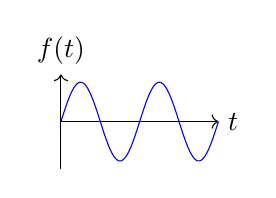
\begin{tikzpicture}[scale=0.5]
    \draw[->] (0,0) -- (4,0) node[right] {$t$};
    \draw[->] (0,-1.2) -- (0,1.2) node[above] {$f(t)$};
    \draw[domain=0:4, samples=100, blue] plot (\x, {sin(180*\x)});
\end{tikzpicture}
} \\ \hline

2. Unit Step Signal & $u(t) = \begin{cases} 1 & t \ge 0 \\ 0 & t < 0 \end{cases}$ & 
\raisebox{-0.8\height}{
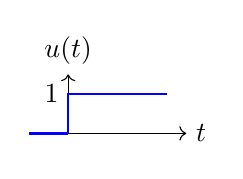
\begin{tikzpicture}[scale=0.5]
    \draw[->] (-1,0) -- (3,0) node[right] {$t$};
    \draw[->] (0,0) -- (0,1.5) node[above] {$u(t)$};
    \draw[thick, blue] (0,0) -- (0,1) -- (2.5,1);
    \draw[thick, blue] (-1,0) -- (0,0);
    \node at (0,1) [left] {1};
\end{tikzpicture}
} \\ \hline

3. Ramp Signal & $r(t) = \begin{cases} t & t \ge 0 \\ 0 & t < 0 \end{cases}$ & 
\raisebox{-0.8\height}{
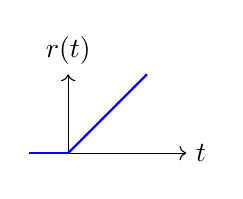
\begin{tikzpicture}[scale=0.5]
    \draw[->] (-1,0) -- (3,0) node[right] {$t$};
    \draw[->] (0,0) -- (0,2) node[above] {$r(t)$};
    \draw[thick, blue] (0,0) -- (2,2);
    \draw[thick, blue] (-1,0) -- (0,0);
\end{tikzpicture}
} \\ \hline

4. Impulse Signal & $\delta(t) = \begin{cases} \infty & t = 0 \\ 0 & t \ne 0 \end{cases}$ & 
\raisebox{-0.8\height}{
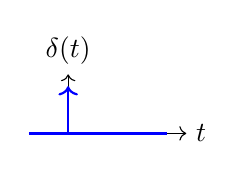
\begin{tikzpicture}[scale=0.5]
    \draw[->] (-1,0) -- (3,0) node[right] {$t$};
    \draw[->] (0,0) -- (0,1.5) node[above] {$\delta(t)$};
    \draw[thick, ->, blue] (0,0) -- (0,1.2);
    \draw[thick, blue] (-1,0) -- (0,0) -- (2.5,0);
\end{tikzpicture}
} \\ \hline
\end{longtable}
\end{center}
\end{solutionbox}

\begin{mnemonicbox}
\mnemonic{Sine Oscillates, Step Jumps, Ramp Climbs, Impulse Spikes}
\end{mnemonicbox}

\questionmarks{3}{c}{7}
\textbf{OR: Draw and explain Pre emphasis and De emphasis circuit with its need \& characteristic graph. Also compare FM receiver with AM receiver in detail.}

\begin{solutionbox}
\textbf{Pre-emphasis and De-emphasis:}
\begin{itemize}
    \item \textbf{Need}: In FM, high-frequency components of the message signal have a lower modulation index compared to low-frequency components, making them more susceptible to noise (as noise power density increases with frequency in FM demodulator output).
    \item \textbf{Solution}: We artificially boost (amplify) high frequencies at the transmitter (\textbf{Pre-emphasis}) and attenuate them correspondingly at the receiver (\textbf{De-emphasis}) to improve SNR.
\end{itemize}

\textbf{Circuits:}

\begin{center}
\begin{circuitikz}[scale=0.8]
    % Pre-emphasis
    \node at (2, 2.5) {\textbf{Pre-emphasis (Transmitter)}};
    \draw (0,0) node[left] {$V_{in}$} to[short, o-] (1,0); 
    \draw (1,0) -- (1, 1) to[C, l=$C$] (3,1) -- (3,0);
    \draw (1,0) to[R, l=$R_1$] (3,0);
    \draw (3,0) -- (4,0) to[R, l=$R_2$] (4,-2) node[ground] {};
    \draw (3,0) to[short, -o] (5,0) node[right] {$V_{out}$};
    \node at (2.5, -2.5) {Simple Pre-emphasis Network};
\end{circuitikz}
\hfill
\begin{circuitikz}[scale=0.8]
    % De-emphasis
    \node at (2, 2.5) {\textbf{De-emphasis (Receiver)}};
    \draw (0,0) node[left] {$V_{in}$} to[short, o-] (1,0) to[R, l=$R$] (3,0) -- (4,0) to[short, -o] (5,0) node[right] {$V_{out}$};
    \draw (3,0) to[C, l=$C$] (3,-2) node[ground] {};
    \node at (2.5, -2.5) {Simple De-emphasis Network};
\end{circuitikz}
\captionof{figure}{Pre-emphasis and De-emphasis Circuits}
\end{center}

\textbf{Characteristic  Graph:}
\begin{center}
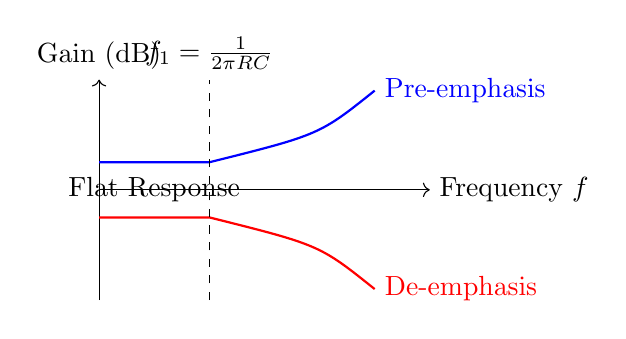
\begin{tikzpicture}[scale=0.7]
    \draw[->] (0,0) -- (6,0) node[right] {Frequency $f$};
    \draw[->] (0,-2) -- (0,2) node[above] {Gain (dB)};
    \draw[thick, blue] (0,0.5) -- (2,0.5) .. controls (4,1) .. (5,1.8) node[right] {Pre-emphasis};
    \draw[thick, red] (0,-0.5) -- (2,-0.5) .. controls (4,-1) .. (5,-1.8) node[right] {De-emphasis};
    \draw[dashed] (2,-2) -- (2,2) node[above] {$f_{1} = \frac{1}{2\pi RC}$};
    \node at (1,0) {Flat Response};
\end{tikzpicture}
\end{center}

\textbf{Comparison of FM and AM Receivers:}
\begin{center}
\begin{tabulary}{\linewidth}{|L|L|L|}
\hline
\textbf{Parameter} & \textbf{AM Receiver} & \textbf{FM Receiver} \\ \hline
1. Operating Frequencies & MF/HF Range (535-1605 kHz) & VHF Range (88-108 MHz) \\ \hline
2. IF Frequency & 455 kHz & 10.7 MHz \\ \hline
3. Bandwidth & 10 kHz & 200 kHz \\ \hline
4. Demodulation & Envelope Detector & Discriminator / Ratio Detector \\ \hline
5. Amplitude Limiter & Not required & Essential to remove amplitude noise \\ \hline
6. Pre/De-emphasis & Not used & Used to improve SNR \\ \hline
7. Audio Quality & Moderate, mono & High fidelity, often stereo \\ \hline
\end{tabulary}
\end{center}
\end{solutionbox}

\begin{mnemonicbox}
\mnemonic{Pre Boosts Highs, De Cuts Them; FM Filters Noise Better Than AM}
\end{mnemonicbox}

\questionmarks{4}{a}{3}
\textbf{Define Image frequency in a radio receiver and explain it with suitable example.}

\begin{solutionbox}
\textbf{Image Frequency}: An unwanted input frequency located equidistant from the Local Oscillator (LO) frequency as the desired signal frequency, which, when mixed with the LO, produces the same Intermediate Frequency (IF).

\textbf{Explanation with Example:}
\begin{itemize}
    \item Let desired Station Frequency $f_s = 1000 \text{ kHz}$.
    \item Standard IF $f_{IF} = 455 \text{ kHz}$.
    \item Local Oscillator Frequency (High side injection) $f_{LO} = f_s + f_{IF} = 1000 + 455 = 1455 \text{ kHz}$.
    \item The mixer produces difference frequencies: $|f_{LO} - f_{in}| = f_{IF}$.
    \item \textbf{Case 1}: $f_{in} = f_s = 1000 \text{ kHz} \Rightarrow |1455 - 1000| = 455 \text{ kHz}$ (Desired).
    \item \textbf{Case 2}: $f_{in} = f_{si} \text{ (Image)} = f_s + 2f_{IF} = 1000 + 2(455) = 1910 \text{ kHz}$.
    \item Check: $|1455 - 1910| = |-455| = 455 \text{ kHz}$.
    \item Thus, if a station exists at 1910 kHz, it will interfere with the 1000 kHz station.
\end{itemize}
Equation: $f_{si} = f_s + 2f_{IF}$
\end{solutionbox}

\begin{mnemonicbox}
\mnemonic{Image In radio Is Interfering 2IF away}
\end{mnemonicbox}

\questionmarks{4}{b}{4}
\textbf{Draw and explain envelope detector circuit for demodulation of Amplitude modulated signal.}

\begin{solutionbox}
\textbf{Envelope Detector Circuit:}

\begin{center}
\begin{circuitikz}[scale=1]
    \draw (0,0) node[left] {AM Input} to[short, o-] (1,0) to[D, l=$D$] (3,0) -- (5,0) to[short, -o] (6,0) node[right] {Audio Output};
    \draw (3,0) to[R, l=$R$, *-*] (3,-2) node[ground] {};
    \draw (4.5,0) to[C, l=$C$, *-*] (4.5,-2) node[ground] {};
\end{circuitikz}
\captionof{figure}{Simple Diode Envelope Detector}
\end{center}

\textbf{Working Principle:}
\begin{enumerate}
    \item \textbf{Rectification}: During the positive half-cycle of the AM input, the diode $D$ becomes forward biased and charges the capacitor $C$ to the peak value of the input voltage.
    \item \textbf{Discharging}: As the input voltage drops below the peak, the diode becomes reverse biased. The capacitor discharges slowly through resistor $R$.
    \item \textbf{Envelope Tracking}: If the $RC$ time constant is chosen correctly, the capacitor voltage follows the envelope of the AM wave (which represents the message signal) rather than the high-frequency RF carrier variations.
    \item \textbf{Time Constant Selection}: The time constant $\tau = RC$ must satisfy:
    \[ \frac{1}{f_c} \ll RC \ll \frac{1}{f_m} \]
    This ensures it filters out the carrier ($f_c$) but retains the message ($f_m$).
\end{enumerate}
\end{solutionbox}

\begin{mnemonicbox}
\mnemonic{Diode Rectifies, RC Smooths Envelope}
\end{mnemonicbox}

\questionmarks{4}{c}{7}
\textbf{Draw block diagram of AM radio receiver and explain working of each block.}

\begin{solutionbox}
\textbf{Superheterodyne AM Receiver Block Diagram:}

\begin{center}
\begin{tikzpicture}[auto, node distance=2.5cm, >=latex]
    \node [gtu block] (ant) {Antenna};
    \node [gtu block, right of=ant] (rf) {RF Amp};
    \node [gtu block, right of=rf] (mixer) {Mixer};
    \node [gtu block, right of=mixer] (if) {IF Amp};
    \node [gtu block, below of=if] (det) {Detector};
    \node [gtu block, left of=det] (af) {AF Amp};
    \node [gtu block, left of=af] (spk) {Speaker};
    \node [gtu block, below of=mixer] (lo) {Local Oscillator};

    \draw [gtu arrow] (ant) -- (rf);
    \draw [gtu arrow] (rf) -- (mixer);
    \draw [gtu arrow] (mixer) -- (if);
    \draw [gtu arrow] (if) -- (det);
    \draw [gtu arrow] (det) -- (af);
    \draw [gtu arrow] (af) -- (spk);
    \draw [gtu arrow] (lo) -- (mixer);
    \draw [dashed] (rf) -- (lo) node[midway, left] {Ganged Tuning};
\end{tikzpicture}
\captionof{figure}{Superheterodyne AM Receiver}
\end{center}

\textbf{Working of Each Block:}
\begin{itemize}
    \item \textbf{RF Amplifier}: Selects the desired station frequency ($f_s$) and rejects others. Improves signal-to-noise ratio.
    \item \textbf{Local Oscillator}: Generates a high-frequency sine wave ($f_{LO}$) such that $f_{LO} = f_s + f_{IF}$. It tracks the tuning of the RF stage.
    \item \textbf{Mixer}: Mixes $f_s$ and $f_{LO}$ to produce the Intermediate Frequency ($f_{IF} = 455 \text{ kHz}$) using the principle of heterodyning (beat frequency).
    \item \textbf{IF Amplifier}: A high-gain tuned amplifier fixed at 455 kHz. It provides most of the receiver's gain and selectivity.
    \item \textbf{Detector}: Demodulates the constant-IF AM signal to recover the original audio message signal. Usually includes AGC (Automatic Gain Control).
    \item \textbf{AF Amplifier}: Amplifies the weak audio signal to a level sufficient to drive the loudspeaker.
    \item \textbf{Speaker}: Transducer that converts electrical audio signals into sound waves.
\end{itemize}
\end{solutionbox}

\begin{mnemonicbox}
\mnemonic{Radio Mixing Intermediate Detected Audio For Speaker}
\end{mnemonicbox}

\questionmarks{4}{a}{3}
\textbf{OR: State and explain Nyquist Criteria for sampling of signal.}

\begin{solutionbox}
\textbf{Nyquist Sampling Theorem:}
\begin{quote}
"A continuous-time signal can be completely reconstructed from its samples if and only if the sampling frequency ($f_s$) is greater than or equal to twice the maximum frequency component ($f_{max}$) present in the signal."
\end{quote}

\textbf{Mathematical Condition:}
\[ f_s \ge 2 f_{max} \]

\textbf{Explanation:}
\begin{itemize}
    \item \textbf{Nyquist Rate}: The minimum sampling rate required, which is $2 f_{max}$.
    \item \textbf{Aliasing}: If $f_s < 2 f_{max}$, the high-frequency components "fold over" into the low-frequency spectrum, causing distortion known as aliasing. The original signal cannot be recovered.
    \item \textbf{Guard Band}: In practice, $f_s$ is chosen slightly higher than $2 f_{max}$ to allow for practical anti-aliasing filters (e.g., $f_s = 44.1 \text{ kHz}$ for audio with $f_{max} = 20 \text{ kHz}$).
\end{itemize}
\end{solutionbox}

\begin{mnemonicbox}
\mnemonic{Sample at least Twice as Fast as Highest Frequency}
\end{mnemonicbox}

\questionmarks{4}{b}{4}
\textbf{OR: Explain slope overload and granular noise for a delta modulation.}

\begin{solutionbox}
In Delta Modulation (DM), the analog signal is approximated by a staircase function with a fixed step size ($\delta$). Two types of quantization errors occur:

\textbf{1. Slope Overload Distortion:}
\begin{itemize}
    \item \textbf{Cause}: Occurs when the analog input signal changes (rises or falls) very rapidly, i.e., it has a high slope.
    \item \textbf{Effect}: The staircase approximation cannot keep up with the steep slope of the input signal because the step size is too small or sampling rate is too low.
    \item \textbf{Remedy}: Increase the step size ($\delta$) or the sampling frequency ($f_s$).
\end{itemize}

\textbf{2. Granular Noise:}
\begin{itemize}
    \item \textbf{Cause}: Occurs when the analog input signal is relatively flat or changes very slowly.
    \item \textbf{Effect}: The staircase output oscillates above and below the true signal level by the step size $\delta$, creating a noise-like variation even when silence exists.
    \item \textbf{Remedy}: Decrease the step size ($\delta$).
\end{itemize}

\textbf{Trade-off}: Increasing step size fixes slope overload but worsens granular noise, and vice versa. \textbf{Adaptive Delta Modulation (ADM)} solves this by varying the step size dynamically.
\end{solutionbox}

\begin{mnemonicbox}
\mnemonic{Slopes Need Bigger Steps, Flats Need Smaller Steps}
\end{mnemonicbox}

\questionmarks{4}{c}{7}
\textbf{OR: Draw and explain PCM transmitter and receiver in detail.}

\begin{solutionbox}
\textbf{Block Diagram of PCM System:}

\begin{center}
\textbf{PCM Transmitter}

\begin{tikzpicture}[auto, node distance=2cm, >=latex]
    \node [gtu block] (source) {Analog Source};
    \node [gtu block, right of=source, node distance=2.5cm] (lpf) {LPF};
    \node [gtu block, right of=lpf, node distance=2.5cm] (sampler) {Sampler};
    \node [gtu block, right of=sampler, node distance=2.5cm] (quant) {Quantizer};
    \node [gtu block, right of=quant, node distance=2.5cm] (enc) {Encoder};
    \node [right of=enc, node distance=2cm] (out) {PCM Out};

    \draw [gtu arrow] (source) -- (lpf);
    \draw [gtu arrow] (lpf) -- (sampler);
    \draw [gtu arrow] (sampler) -- (quant);
    \draw [gtu arrow] (quant) -- (enc);
    \draw [gtu arrow] (enc) -- (out);
\end{tikzpicture}

\vspace{0.5cm}
\textbf{PCM Receiver}

\begin{tikzpicture}[auto, node distance=2cm, >=latex]
    \node [left of=dec, node distance=2cm] (in) {PCM In};
    \node [gtu block] (dec) {Decoder};
    \node [gtu block, right of=dec, node distance=3cm] (recon) {Reconstruction Filter / LPF};
    \node [right of=recon, node distance=3cm] (dest) {Analog Out};

    \draw [gtu arrow] (in) -- (dec);
    \draw [gtu arrow] (dec) -- (recon);
    \draw [gtu arrow] (recon) -- (dest);
\end{tikzpicture}
\captionof{figure}{Pulse Code Modulation (PCM) Block Diagram}
\end{center}

\textbf{Explanation of Blocks:}
\begin{enumerate}
    \item \textbf{Low Pass Filter (Anti-aliasing)}: Band-limits the input signal to $f_{max}$ to strictly satisfy Nyquist criteria ($f_s \ge 2 f_{max}$).
    \item \textbf{Sampler (Sample \& Hold)}: Discretizes the specific time instants. Converts continuous-time signal to discrete-time PAM (Pulse Amplitude Modulation) pulses.
    \item \textbf{Quantizer}: Discretizes the amplitude. Approximates each sample value to the nearest standard voltage level from a finite set of $L$ levels. This introduces Quantization Noise.
    \item \textbf{Encoder}: Converts each quantized level into a unique $n$-bit binary code word (e.g., 01101).
    \item \textbf{Decoder}: Used at the receiver to convert the binary stream back into discrete voltage levels (DAC operation).
    \item \textbf{Reconstruction Filter}: A low-pass filter that smooths the staircase output of the decoder to recover the original continuous analog signal.
\end{enumerate}
\end{solutionbox}

\begin{mnemonicbox}
\mnemonic{Sample, Quantize, Encode; Decode, Convert, Reconstruct}
\end{mnemonicbox}

\questionmarks{5}{a}{3}
\textbf{Define Bit, Bit rate and Baud rate with suitable example.}

\begin{solutionbox}
\begin{itemize}
    \item \textbf{Bit}: The fundamental unit of digital information, representing a binary state of 0 or 1.
    \item \textbf{Bit Rate ($R_b$)}: The speed of data transfer, measured as the number of bits transmitted per second.
        \item Unit: bps (bits per second).
        \item Example: If a system transmits '101' in 1 second, $R_b = 3$ bps.
    \item \textbf{Baud Rate}: The rate of signal changes per second (symbol rate).
        \item Unit: Baud.
        \item Relationship: $R_b = \text{Baud Rate} \times \text{bits per symbol}$.
        \item Example: In QPSK Modulation, each symbol carries 2 bits. If Baud Rate is 1000 Baud, Bit Rate is 2000 bps.
\end{itemize}
\end{solutionbox}

\begin{mnemonicbox}
\mnemonic{Bits Build Data, Baud Brings Symbols}
\end{mnemonicbox}

\questionmarks{5}{b}{4}
\textbf{Define multiplexing. State its types. Explain Frequency division multiplexing with suitable diagram.}

\begin{solutionbox}
\textbf{Multiplexing}: The process of simultaneously transmitting multiple message signals over a single communication channel without interference.

\textbf{Types:}
\begin{enumerate}
    \item Frequency Division Multiplexing (FDM) - Analog
    \item Time Division Multiplexing (TDM) - Digital/Analog
    \item Wavelength Division Multiplexing (WDM) - Optical
\end{enumerate}

\textbf{Frequency Division Multiplexing (FDM):}

\begin{center}
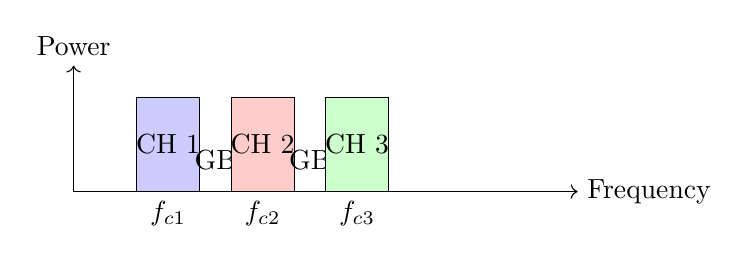
\begin{tikzpicture}[scale=0.8]
    \draw[->] (0,0) -- (8,0) node[right] {Frequency};
    \draw[->] (0,0) -- (0,2) node[above] {Power};
    
    % Channel 1
    \draw[fill=blue!20] (1,0) rectangle (2,1.5);
    \node at (1.5, 0.75) {CH 1};
    \node[below] at (1.5,0) {$f_{c1}$};
    
    % Guard Band
    \node at (2.25, 0.5) {GB};
    
    % Channel 2
    \draw[fill=red!20] (2.5,0) rectangle (3.5,1.5);
    \node at (3, 0.75) {CH 2};
    \node[below] at (3,0) {$f_{c2}$};
    
    % Guard Band
    \node at (3.75, 0.5) {GB};
    
    % Channel 3
    \draw[fill=green!20] (4,0) rectangle (5,1.5);
    \node at (4.5, 0.75) {CH 3};
    \node[below] at (4.5,0) {$f_{c3}$};
    
\end{tikzpicture}
\captionof{figure}{Spectrum of FDM System}
\end{center}

\textbf{Explanation:}
\begin{itemize}
    \item The total bandwidth of the channel is divided into non-overlapping frequency bands.
    \item Each user signal modulates a different carrier frequency ($f_{c1}, f_{c2}, \dots$).
    \item \textbf{Guard Bands} (GB) are unused frequency gaps kept between channels to prevent crosstalk overlap.
    \item All signals are transmitted simultaneously.
    \item Used in FM/AM Radio broadcasting and Cable TV.
\end{itemize}
\end{solutionbox}

\begin{mnemonicbox}
\mnemonic{Frequency Divides Multiple Signals Simultaneously}
\end{mnemonicbox}

\questionmarks{5}{c}{7}
\textbf{Draw and explain basic PCM-TDM diagram with diagram.}

\begin{solutionbox}
\textbf{PCM-TDM System:}
Time Division Multiplexing (TDM) is often used with Pulse Code Modulation (PCM) to transmit multiple digitized voice/data channels over a single link.

\begin{center}
\begin{tikzpicture}[auto, node distance=2cm, >=latex]
    % Inputs
    \node (in1) {Analog 1};
    \node [below of=in1, node distance=1cm] (in2) {Analog 2};
    \node [below of=in2, node distance=1cm] (inN) {Analog N};
    
    % LPFs
    \node [gtu block, right of=in1, node distance=2.5cm] (lpf1) {LPF};
    \node [gtu block, right of=in2, node distance=2.5cm] (lpf2) {LPF};
    \node [gtu block, right of=inN, node distance=2.5cm] (lpfN) {LPF};
    
    % Mux (Commutator)
    \node [gtu block, right of=lpf2, node distance=3cm, minimum height=3cm] (mux) {Commutator (MUX)};
    
    % Common PCM Path
    \node [gtu block, right of=mux, node distance=3cm] (pcm) {ADC (PCM Encoder)};
    \node [right of=pcm, node distance=2.5cm] (out) {PCM-TDM Stream};
    
    % Connections
    \draw [gtu arrow] (in1) -- (lpf1);
    \draw [gtu arrow] (in2) -- (lpf2);
    \draw [gtu arrow] (inN) -- (lpfN);
    
    \draw [gtu arrow] (lpf1) -- (mux.west |- lpf1);
    \draw [gtu arrow] (lpf2) -- (mux.west |- lpf2);
    \draw [gtu arrow] (lpfN) -- (mux.west |- lpfN);
    
    \draw [gtu arrow] (mux) -- (pcm) node[midway, above] {PAM Stream};
    \draw [gtu arrow] (pcm) -- (out);

\end{tikzpicture}
\captionof{figure}{PCM-TDM Transmitter Block Diagram}
\end{center}

\textbf{Operation:}
\begin{enumerate}
    \item \textbf{Input Filtering}: Each analog input is passed through a Low Pass Filter (LPF) to restrict bandwidth.
    \item \textbf{Commutation (Multiplexing)}: An electronic switch (commutator) connects to each input sequentially at a sampling rate $f_s$. This creates an interleaved train of PAM pulses.
    \item \textbf{Encoding}: This single PAM stream is fed to a PCM Encoder (ADC), which quantizes and converts each pulse into an $n$-bit digital code.
    \item \textbf{Transmission}: The resulting high-speed digital stream contains bits from Channel 1, then Channel 2, etc., in a repeating frame structure.
    \item \textbf{Frame}: One complete cycle of scanning all inputs constitutes a TDM Frame. Synchronization bits are usually added to identify frame start.
\end{enumerate}
\end{solutionbox}

\begin{mnemonicbox}
\mnemonic{Pulse Code TDM: Sample, Quantize, Encode, Multiplex}
\end{mnemonicbox}

\questionmarks{5}{a}{3}
\textbf{OR: State types of TDM and explain any one of them.}

\begin{solutionbox}
\textbf{Types of TDM:}
\begin{enumerate}
    \item Synchronous TDM
    \item Asynchronous TDM (or Statistical TDM)
\end{enumerate}

\textbf{Synchronous TDM:}
\begin{itemize}
    \item \textbf{Concept}: Each input source is assigned a fixed time slot in every frame, regardless of whether the source has data to send or not.
    \item \textbf{Operation}: The multiplexer scans inputs in a round-robin fashion. If a device is idle, its time slot is transmitted empty (wasted bandwidth).
    \item \textbf{Advantage}: Simple design, no addressing overhead needed for data fragments (position determines owner).
    \item \textbf{Disadvantage}: Inefficient bandwidth usage if many devices are idle.
\end{itemize}
\end{solutionbox}

\begin{mnemonicbox}
\mnemonic{Synchronous Slots Stay Steady}
\end{mnemonicbox}

\questionmarks{5}{b}{4}
\textbf{OR: Explain TDM. Also State its advantages and disadvantages.}

\begin{solutionbox}
\textbf{Time Division Multiplexing (TDM):}
A digital/analog technique where multiple low-speed signals are interleaved in time to share a single high-speed transmission channel. The time axis is divided into slots, and each user gets the full bandwidth for a fraction of time.

\textbf{Advantages:}
\begin{itemize}
    \item No crosstalk between channels (separated in time).
    \item Utilizes the full bandwidth of the channel.
    \item Circuitry is digital, reliable, and easy to integrate (VLSI).
    \item Flexible: Can handle different data rates with buffering.
\end{itemize}

\textbf{Disadvantages:}
\begin{itemize}
    \item Requires strict \textbf{Synchronization} between transmitter and receiver.
    \item Complexity in clock recovery and framing circuits.
    \item Bandwidth waste in Synchronous TDM if channels are inactive.
    \item Propagation delay affects timing.
\end{itemize}
\end{solutionbox}

\begin{mnemonicbox}
\mnemonic{Time Divided Multiple signals Save costs But Need Precise timing}
\end{mnemonicbox}

\questionmarks{5}{c}{7}
\textbf{OR: State desirable properties of line coding. Draw waveform in time relation for unipolar RZ, Polar NRZ, and Manchester line coding for a 8 bit digital data 01001110.}

\begin{solutionbox}
\textbf{Desirable Properties of Line Coding:}
\begin{enumerate}
    \item \textbf{Self-Synchronization}: Enough transitions for clock recovery.
    \item \textbf{No DC Component}: To allow AC coupling (transformers/capacitors).
    \item \textbf{Error Detection}: Capability to detect bit errors.
    \item \textbf{Bandwidth Efficiency}: Should use minimum channel bandwidth.
    \item \textbf{Low cross-talk}: Reduced interference.
\end{enumerate}

\textbf{Line Coding Waveforms for Data: 0 1 0 0 1 1 1 0}

\begin{center}
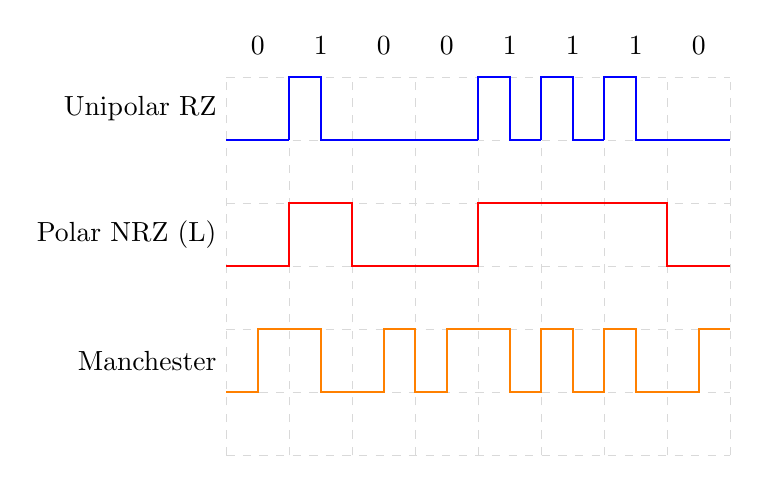
\begin{tikzpicture}[scale=0.8]
    % Grid
    \draw[help lines, dashed, gray!30] (0,0) grid (8,6);
    
    % Bit labels
    \foreach \x/\bit in {0.5/0, 1.5/1, 2.5/0, 3.5/0, 4.5/1, 5.5/1, 6.5/1, 7.5/0} {
        \node at (\x, 6.5) {\bit};
    }
    
    % Unipolar RZ
    \node[left] at (0, 5.5) {Unipolar RZ};
    \draw[thick, blue] (0,5) -- (0.5,5) -- (0.5,5) -- (1,5)
                      (0,5) -- (1,5)
                      (1,5) -- (1,6) -- (1.5,6) -- (1.5,5) -- (2,5)
                      (2,5) -- (3,5)
                      (3,5) -- (4,5)
                      (4,5) -- (4,6) -- (4.5,6) -- (4.5,5) -- (5,5)
                      (5,5) -- (5,6) -- (5.5,6) -- (5.5,5) -- (6,5)
                      (6,5) -- (6,6) -- (6.5,6) -- (6.5,5) -- (7,5)
                      (7,5) -- (8,5);

    % Polar NRZ
    \node[left] at (0, 3.5) {Polar NRZ (L)};
    \draw[thick, red] (0,3) -- (1,3)
                     -- (1,4) -- (2,4)
                     -- (2,3) -- (3,3)
                     -- (4,3)
                     -- (4,4) -- (5,4)
                     -- (6,4)
                     -- (7,4)
                     -- (7,3) -- (8,3);

    % Manchester
    \node[left] at (0, 1.5) {Manchester};
    \draw[thick, orange] (0,1) -- (0.5,1) -- (0.5,2) -- (1,2)
                       -- (1,2) -- (1.5,2) -- (1.5,1) -- (2,1)
                       -- (2,1) -- (2.5,1) -- (2.5,2) -- (3,2)
                       -- (3,1) -- (3.5,1) -- (3.5,2) -- (4,2)
                       -- (4,2) -- (4.5,2) -- (4.5,1) -- (5,1)
                       -- (5,2) -- (5.5,2) -- (5.5,1) -- (6,1)
                       -- (6,2) -- (6.5,2) -- (6.5,1) -- (7,1)
                       -- (7,1) -- (7.5,1) -- (7.5,2) -- (8,2);

\end{tikzpicture}
\captionof{figure}{Line Coding Waveforms}
\end{center}
\end{solutionbox}

\begin{mnemonicbox}
\mnemonic{Unipolar Rises then Zeros, Polar Never Returns, Manchester Always Transitions}
\end{mnemonicbox}

\end{document}
